
% Introduce the different experiments
% If experiment refer to each other, possibly also mention that here.

\chapter{Results \& Discussion}
The experiments performed during the project have led to many interesting results. Every experiment performed have had great impact on the AIs final performance (g: EVALUERING/ANALYS?). Either by presenting the problems and complications that the AI faces during learning or by providing a way to evaluate whether or not the modelling of the environment is sufficient.

This chapter presents and discusses the results that have been achieved during the project. The chapter is divided into sections by experiments performed. Each section presents results as well discussion and reflections about the experiments. The sections also introduce how different experiments and their results relate to each other. The order in which these results are presented follows the order in which conclusions were drawn and the project progressed (g: FOKUSERA PÅ LÄSAREN, INTE PÅ VÅRT PROJECT, TROR JAG). Thus one should get a general understanding of the AIs performance improvements during the project from this chapter.

% ----------------------------------------------------------------------------------------
% Refer to the description in method
% Present the results of the experiment
    % - What did it do?
    % - Fitness
    % - Generations required before results
    % - (Population)
% Analyse the results and the meanings behind them.
    % - Was it a good result? Why/Why not?
    % - What conclusions can be drawn from the results?
    % - How could we modify this experiment in order to get additional meaningful results?
% ----------------------------------------------------------------------------------------

% refer to the description in Method
% example: did it help to help in any way
% example: present data
% example: did the hypothesis work
\section{Fixed speed}
% constant speed -> focus on steering, one variable
% gradually increasing speed, method?
% increasing speed -> push the limits 

KEY FINDINGS: INTERPRET DATA WELL, FIND COMPLEX BEHAVIOUR, NOT OBSERVED TO OPTIMISE EVERYTHING IN THE SAME SOLUTION(?), HARD TO SEPARATE SIMILAR SCENARIOS, ...

By locking the speed of the car to a constant value, conclusions about the AIs ability to steer the car could be drawn. The constant speed was gradually increased with the goal to force the AI to modify the race line such that it takes wider corners, making it possible for the car to go around the track in such an efficient way as possible, given the current speed.

Noteworthy is that after the car completes a track, rewarding it for improved time or improved distance driven is analogous. Since the car is driving at a constant speed, this will only result in a shorter distance being driven to get around the track.

The experiment was performed in two ways, one where the AI can look further down the track and one where it only has local knowledge about the track. Results for each of these sub-experiments are presented in the subsections below.

% By locking the speed of the car to a constant value, this experiment aimed to evaluate the networks ability to steer the car. The speed was initially set to a value that was known to be low enough for the car to be able to take a lap by driving in the middle of the track at all times. The speed was increased gradually, trying to force the AI to take wider race line in order to get around the track with the higher speed.

% After it completes a track, rewarding it for improved time or improved distance driven is analogous, since it drive at a constant speed.

% NOTE: I am not certain that some results are actually correct in this section. Does it actually stick to the middle? I do not believe that I had that behaviour when I ran the experiment on the cloud computer. Can't visualise it atm though.
\subsection{Only local perception}
Providing the system only with local perception, as explained in section 3.6.1, present successful and interesting results. The system tries to position the car in the middle of the track at all times. Given that the system only has knowledge about the local relation between the car and the track, this behaviour is reasonable and to be expected. On the straights, this behaviour works well. However the car eventually encounters a corner, which causes the middle of the track to shift.

When the AI is not provided with any information about how the track looks in front of the car, the car sticks to the middle of the track. Since the AI only has knowledge about the track in a small space around the car, it never adjusts for corners before they are actually next to the car. This means that when the car eventually encounters a corner, it will appear as though the car is no longer in the middle of the track. At this point the AI tries to recover the car and position it in the middle of the track again. This lead to late reactions, making it impossible to get past tight curves if the speed was too high simply by reacting to the distance from the middle as the curve appears.

The AI tries to compensate for these late reactions by increasing the amount of steering applied. This causes the car to oscillate around the tracks mid line. The oscillation occasionally helps the car to position itself correctly before a tough curve. Which further helps the car to complete the corner. The oscillation only occurs after the first curvature on the track, since that is the point in which it has to start compensating. Eventually the AI learned to minimise the oscillation and the car seems to simply stick to the middle of the track.

When the cars speed was pushed to values that requires the car to take wider curves then sticking to the middle, the car failed to make a complete lap. The amount of steering required in order to complete certain curves from the middle of the track is simply larger than the available turning radius, and the oscillation required to compensate for this forces the car to drive outside of the track or failing other corners.

The speed was initially set to 10 m/s, which resulted in the car managing to take a lap on generation 2. The speed was then gradually increased to 11.6, 11.7, 11.75 and 15 m/s. At 11.6m/s the car managed to make a complete lap after 5 generations. At 11.7 m/s, the car managed to make a complete lap at generation 22. Further increasing the speed resulted in the car not taking a complete lap.

% Storlek och vilka indata som används.
%[Network structure...]

% TODO: Add some more reflections
The only way it can know there is a curve, is if it find itself away from the middle. It is therefore impossible for it to sophistically prepare for an approaching curve. The only way it improved after a certain degree was if it found an accidental oscillation, where it started to steer before the start of a curve. It is an unstable solution which did not work for several subsequent difficult curves.

[Does it behave differently with edge distance data instead or in addition to distance to middle data? Will it stick to another lateral position than the middle?]

% OLD TEXT:

% When the constant speed was increased, the car started to oscillate around the mid line of the track. The oscillation however only occurred after the first curve in the track, which was interesting. The oscillation sometimes helped the car to position itself in a better way for a tough curve, which in turn helped it to complete that curve. Oscillation will however cause the car to drive a longer distance, compared to driving in a straight line. After completing the track, if the oscillation was not needed for taking a specific curve, it always stopped. The network managed to learn to make it stable. 

% The car stick to the middle of the track. If it drives in to a curve and appear away from the middle, it tries to recover. If it approached a tight curve, it would not perceive the curve until it suddenly appear to drive away from the middle. This lead to late reactions, making it impossible to get past curves if they were to tight or the speed was too high.

% It usually resulted in oscillations around the mid line, usually after some disturbance like the initial curved. Some times the oscillation made it get in better position for a difficult curve, allowing it to complete the curve better. 

% Oscillation will cause the car to drive longer than if it would drive straight. After completing the track, if the oscillation was not needed for taking a specific curve, it always stopped. The network managed to learn to make it stable. 

% The only way it can know there is a curve, is if it find itself away from the middle. It is therefore impossible for it to sophistically prepare for an approaching curve. The only way it improved after a certain degree was if it found an accidental oscillation, an unstable solution which did not work for several subsequent difficult curves.

% Training times...

% Network structure... 

% [Does it behave differently with edge distance data instead or in addition to distance to middle data? Will it stick to another lateral position than the middle?]


\subsection{Local perception and track curvature}

% Ser vi något intressant om vi ökar hastigheten
% Beteende:
% - Klarar högre hastigheter
% - Svänger före kurvorna
% - Tar mer höjd inför kurvorna
% - 

% Beteendeanalys:
% - tolkar datan bra
% - beter sig i stora delar som man kan förvänta sig
% - Begränsad av hastigheten och bilens prestanda, som vi ser när man ökar hastigheten att beteendet blir "sämre"

% Data:
% - när tar den ett varv
% - när blir det optimalt
% - storlek på nätverket och vilka indata

% Analys:
% - Vilken data användes för det här problemet/beteendet?
% - Hur lyckades NEAT hitta något
% - Kan den lära sig flera saker samtidigt?

It is interesting to investigate how much the AI can manage to improve if it has access to the curvature of the track ahead. 

We found solutions that managed to complete the track with speeds up to 12.1 m/s, compared to 11.7 m/s without the track curvature data. The difference in speed may seem small, but the difference in behaviour is substantial.

What these solutions generally do is that they position themselves well before a curve, to compensate for the larger turning radius. They also start to steer before the curve actually start.

The speed that provided the most correctly looking race lines was 12.0 m/s. At that speed the AI had to push the limits in order to manage the toughest chicane. When the speed increased, the AI had to start turning very late in the chicane, to make a little more space for the following curve. This made it less interesting to investigate further, since that behaviour resembled real behaviour less.

% Check for longer training sessions
Each of the solutions found showed some typical characteristics. If one solution managed to drive tightly to the inner side in the toughest curve or positioned itself extremely before a curve, it also showed that tendency for all other mayor curves. On the contrary, if it turned late in the tough curves, it also did it for the other curves too.

%Check for longer training sessions
The recurrent characteristics in the behaviour for a particular solution often had one limitation, that they failed to manage simpler as efficient as the tough curves. If the solution managed to take the tough curve, near optimally, we never observed that it also managed to take the simpler curves as efficiently. For example, for the lightly turning curves, the car always drove a few meters from the edge of the track, even if it certainly had traction to stay closer. 

%Check for longer training sessions
It seemed like it did not learn to distinguish properly between the different difficulties, and simple did the same behaviour in miniature. Worth noting was that these training sessions lasted for only about 2-600 generations. We have not proven that it is not possible if one trains for longer.

The best network found for the speed 50.0 had fitness 5821.93. It had a total of 9 hidden nodes, a total of 20 edges, 8 edges within the hidden layer, 4 to output nodes, 9 of the input nodes and bias was connected (0, 1, 3, 4, 5, 7, 8, 10, 13, 15) (bias, distance to middle, distance to right edge, angle to mid line, curve data points 10m 42m 66m 144m 397m and the segment sum of the first four points in the region 10-66m) (Remember to check which edges are enabled!)


\subsection{Shortest path}

The fastest route for a car that moves forward with a constant speed is the shortest one. This means that the only way for a genome to increase its fitness once it completes the circuit is to decrease the distance driven around the track.  

The result show that after the algorithm finds specimens that are able to complete the circuit, the gene pool continues to improve. The path around the circuit is shortened to a great extent. The difference in length of the raceline and the midline of the circuit is significant. 

The optimal behaviour is intuitively to always drive on the inner curves and to drive a straight line between the curves where it has to turn. Small variations on the curvature should not matter, if the edge does not intersect with the path the car drives.

The car follow the key behaviour aspects, but not to the extent that the path is optimal. We can see that it drives tightly to the inner side for very tight curves, but not for low intensity curves.

Training times...

Network structure...


%\section{(Existing steering controller)}
% refer to the description in Method
% example: did it help to help in any way
% example: present data
% example: did the hypothesis work

\section{Steer and speed control}
%KEY FINDINGS: SIGNIFICANT INCREASE IN COMPUTATIONAL COMPLEXITY, FEWER OPTIMAL ASPECTS(?), ...

% refer to the description in Method
% example: did it help to help in any way
% example: present data
% example: did the hypothesis work

% Beteendeanalys
% - it do optimise for time!
% training, data,

% Analysis
% - Similar times as for the fixed speed
% - How do the behaviour/ performance differ to the fixed speed. 
% - Longer training time => more complex
% - Can it manage to learn many components of the behaviour at the same time? One component only may make the performance worse
%

When the genomes are given steering and breaking as a second output, the complexity of the computations increase significantly according to the results. It takes this experiment 506 generations until a genome can complete a single lap around the track. This genome have the ability to both use the break and throttle, but would hold a lower average speed than the best genomes in the corresponding constant speed experiment.

After a genome manages to complete a lap around the track, the data shows that the training process actually manages to find genomes that can complete the track in less time. 


\begin{figure}[h]
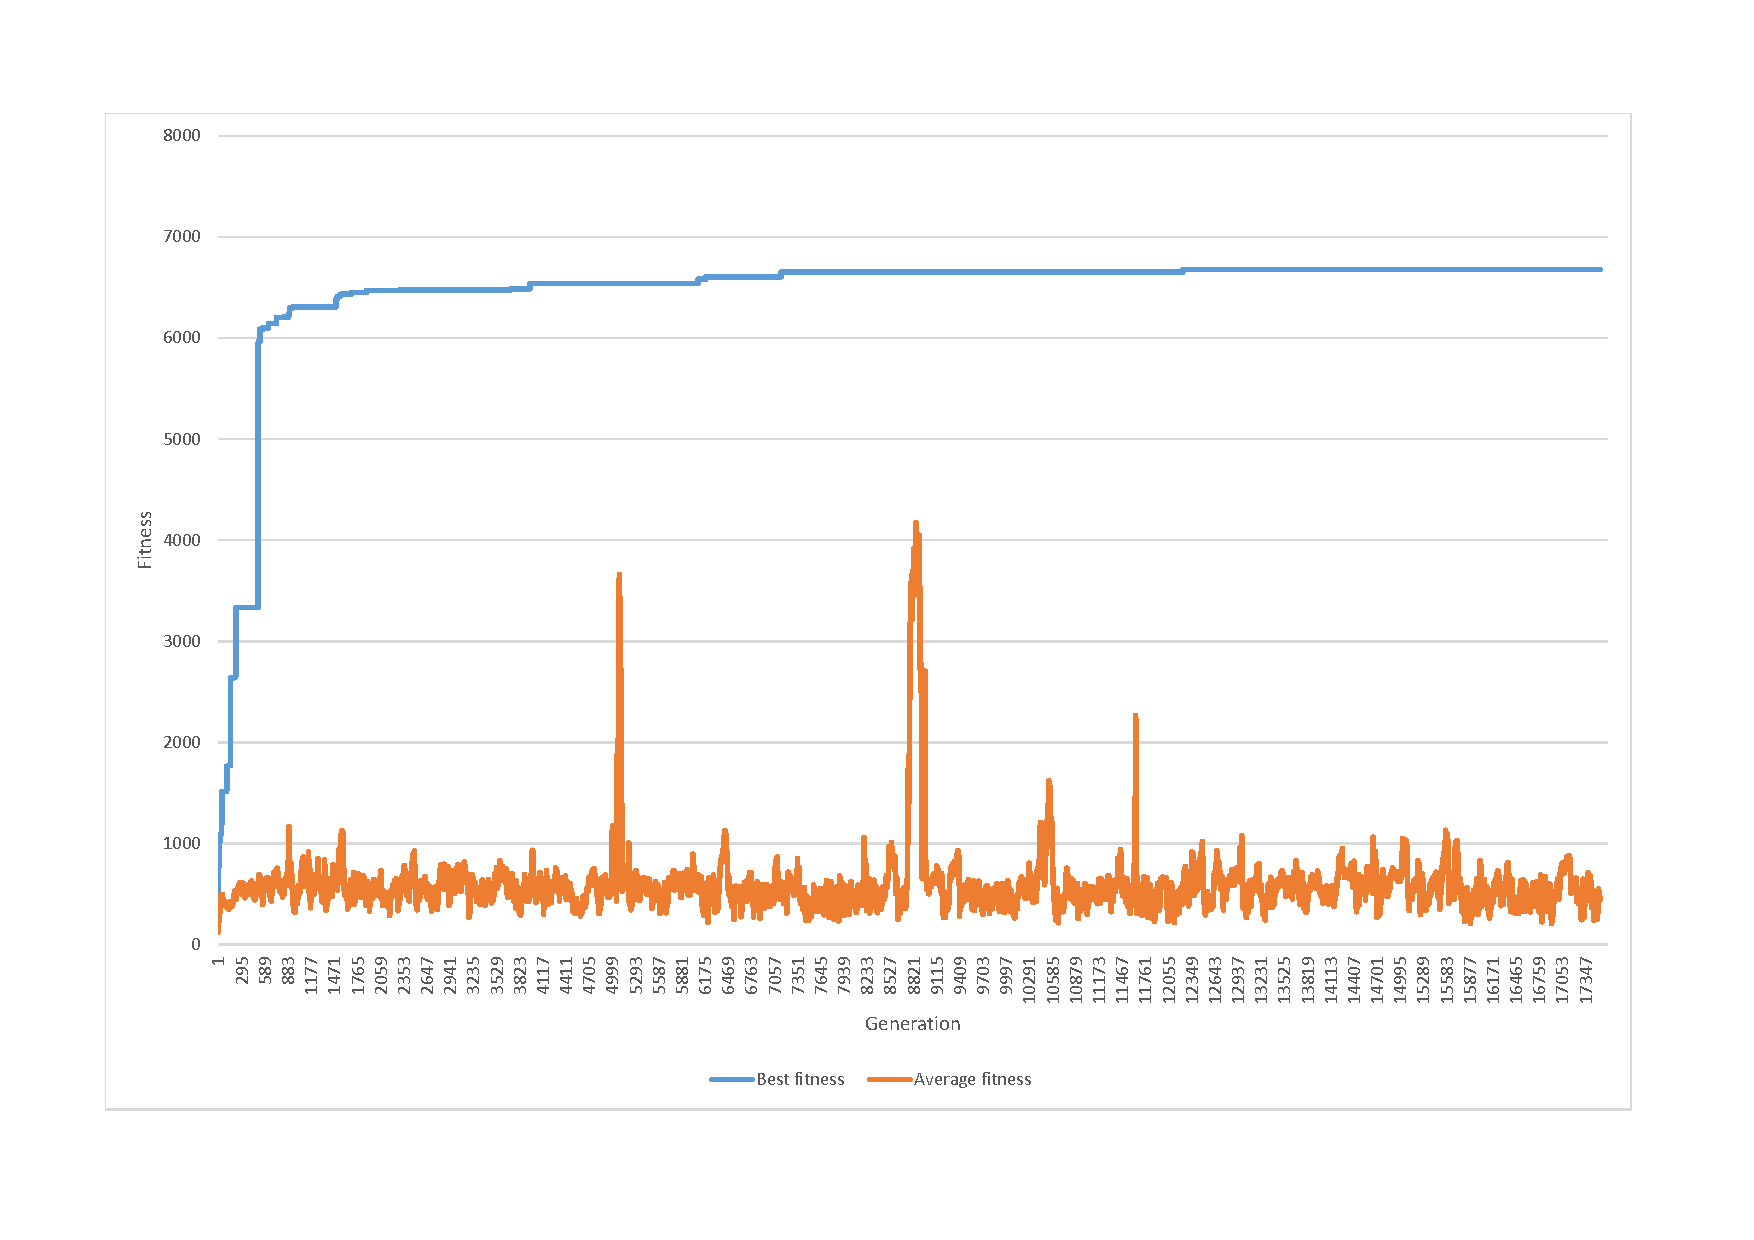
\includegraphics[width=\textwidth]{report/images/graphs/fitness}
\centering
\caption{Showing best fitness and average fitness of each generation}
\end{figure}

As can be seen in the graph above (insert proper tagging), the car AI creates a genome that reaches a fitness higher than the termination distance at 5200 in relatively few generations. Once this fitness level of 5200 is reached, the algorithm tries to optimise the time spent driving. The p

\section{Single short track segment}

% \section{Multiple short track segments}

\section{Mirror track}
%Train at one track, then drive it on the mirrored track


%- If it is trained for certain tracks, can it manage others?


\section{Summary of results}
